\documentclass[10pt,a4paper,spanish]{report}

\usepackage[spanish]{babel}
\usepackage[utf8]{inputenc}
\usepackage{amsmath, amsthm}
\usepackage{amsfonts, amssymb, latexsym}
\usepackage{enumerate}
\usepackage[official]{eurosym}
\usepackage{graphicx}
\usepackage[usenames, dvipsnames]{color}
\usepackage{colortbl}
\usepackage{multirow}
\usepackage{fancyhdr}
\usepackage[all]{xy}
\usepackage{pgfplots}
\usepackage{algpseudocode}
\usepackage{listings}
\usepackage{titlesec}

\pgfplotsset{compat=1.5}

% a4large.sty -- fill an A4 (210mm x 297mm) page
% Note: 1 inch = 25.4 mm = 72.27 pt
%       1 pt = 3.5 mm (approx)

% vertical page layout -- one inch margin top and bottom
\topmargin      0 mm    % top margin less 1 inch
\headheight     0 mm    % height of box containing the head
\headsep       10 mm    % space between the head and the body of the page
\textheight   250 mm
\footskip      14 mm    % distance from bottom of body to bottom of foot

% horizontal page layout -- one inch margin each side
%\oddsidemargin    0   mm    % inner margin less one inch on odd pages
%\evensidemargin   0   mm    % inner margin less one inch on even pages
%\textwidth      159.2 mm    % normal width of text on page

\usepackage[math]{iwona}
\usepackage[T1]{fontenc}
\usepackage{inconsolata}

\usepackage[pdftex, bookmarks=true,
	bookmarksnumbered=false, % true means bookmarks in
	% left window are numbered
	bookmarksopen=false,     % true means only level 1
	% are displayed.
	colorlinks=true,
linkcolor=webblue]{hyperref}

\definecolor{webgreen}{rgb}{0, 0.5, 0} % less intense green
\definecolor{webblue}{rgb}{0, 0, 0.5}  % less intense blue
\definecolor{webred}{rgb}{0.5, 0, 0}   % less intense red
\definecolor{dblackcolor}{rgb}{0.0,0.0,0.0}
\definecolor{dbluecolor}{rgb}{.01,.02,0.7}
\definecolor{dredcolor}{rgb}{0.8,0,0}
\definecolor{dgraycolor}{rgb}{0.30,0.3,0.30}

\newcommand{\HRule}{\rule{\linewidth}{0.5mm}} % regla horizontal para  el titulo

\pagestyle{fancy}
%con esto nos aseguramos de que las cabeceras de capítulo y de sección vayan en minúsculas

\renewcommand{\chaptermark}[1]{%
	\markboth{#1}{}}
\renewcommand{\sectionmark}[1]{%
	\markright{\thesection\ #1}}
\fancyhf{} %borra cabecera y pie actuales
\fancyhead[LREO]{\bfseries\thepage}
\fancyhead[LO]{\bfseries\leftmark}
\renewcommand{\headrulewidth}{0.5pt}
\renewcommand{\footrulewidth}{0pt}
\addtolength{\headheight}{0.5pt} %espacio para la raya
\fancypagestyle{plain}{%
	\fancyhead{} %elimina cabeceras en páginas "plain"
	\renewcommand{\headrulewidth}{0pt} %así como la raya
}

%%%%% Para cambiar el tipo de letra en el título de la sección %%%%%%%%%%%
\usepackage{sectsty}
\chapterfont{\fontfamily{pag}\selectfont} %% for chapter if you want
\sectionfont{\fontfamily{pag}\selectfont}
\subsectionfont{\fontfamily{pag}\selectfont}
\subsubsectionfont{\fontfamily{pag}\selectfont}
\titleformat{\chapter}{\normalfont\Huge}{}{0pt}{\Huge} % Capítulos sin "Capítulo x" encima del título

\renewcommand{\labelenumi}{\arabic{enumi}. }
\renewcommand{\labelenumii}{\labelenumi\alph{enumii}) }
\renewcommand{\labelenumiii}{\labelenumii\roman{enumiii}: }

\title{Seguridad y Protección de Sistemas Informáticos \\
Criptosistemas Asimétricos}
\author{David Sánchez Jiménez}

\begin{document}
\begin{titlepage}
 \begin{center}
  \HRule \\[0.8cm]
  \textsc{\huge Seguridad y Protección \\ de Sistemas Informáticos \\[0.5cm] Criptosistemas Asimétricos}\\[1.6cm]
  \HRule \\[1cm]
  \begin{flushleft}
   \emph{Hecho por:}\\
   David Sánchez Jiménez
  \end{flushleft}
  \vspace{12cm}
  \large{\today}\\
  \vspace{0.5cm}
  \htmladdnormallink{
\includegraphics[width=2cm]{Imagenes/88x31.png}}
  {http://creativecommons.org/licenses/by-nc/4.0/}\\[0.5cm]
  \texttt{Prácticas de Seguridad y Protección de Sistemas Informáticos\\ by
   \href{mailto:dasaji92@gmail.com}{David Sánchez Jiménez} is licensed under a \htmladdnormallink{Creative Commons Reconocimiento-NoComercial-CompartirIgual 4.0 Internacional License}
   {http://creativecommons.org/licenses/by-nc/4.0/}}.\\[3mm]
 \end{center}
\end{titlepage}

\tableofcontents
\newpage

% ----------------------------------------------------------------
\chapter{Ejercicio 1}

\section{Enunciado}
\noindent
Cread una autoridad certificadora, En este caso se permitirá el uso de openssl ca frente a CA.pl, aunque este último comando es admisible.

\section{Respuesta}
\noindent
Para la creación de la autoridad certificadora primero es necesario crear la siguiente estructura de carpetas y archivos.

\begin{figure}[!hbp]
 \centering  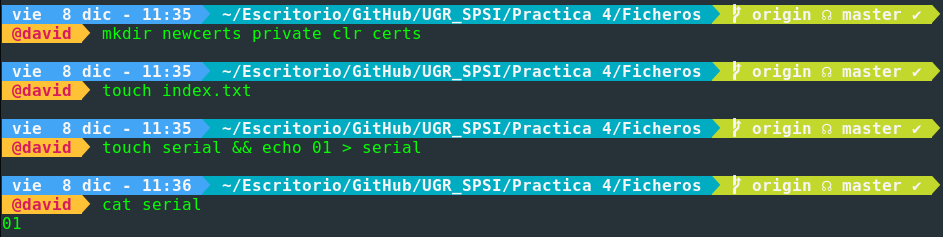
\includegraphics[width=1\textwidth]{./Imagenes/1_1.png}
\end{figure}

\noindent
A continuación busco el archivo openssl.cnf para realizar una copia en el directorio de trabajo y poder modificarlo. A este archivo le he llamado ca.cnf.

\begin{figure}[!hbp]
 \centering  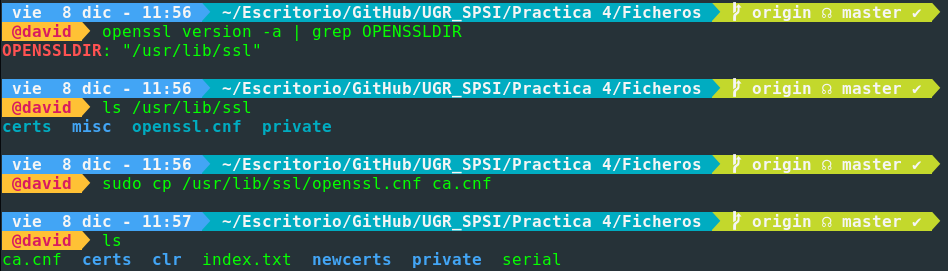
\includegraphics[width=1\textwidth]{./Imagenes/1_2.png}
\end{figure}

\noindent
Una vez tengo el archivo ca.cnf en mi directorio de trabajo paso a modificar el contenido de este. Los parametros modificados son:

\begin{itemize}
 \item En el apartado [ CA\_default ] modifico el parámetro dir	= ./demoCA cambiandolo a dir	= . para que el dir sea el directorio en el que estoy trabajando.
 \item En el apartado [ CA\_default ] modifico el parámetro default\_md	= default cambiandolo a default\_md	= sha256 para que por defecto utilice sha256.
 \item En el apartado [ policy\_match ] modifico el parámetro commonName	= supplied cambiandolo a commonName	= optional.
\end{itemize}

\newpage
\noindent
Por último, creo la clave que usará la autoridad certificadora:

\begin{figure}[!hbp]
 \centering  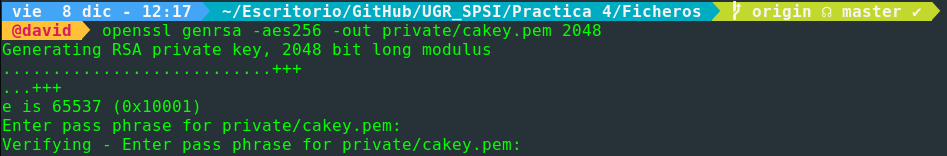
\includegraphics[width=1\textwidth]{./Imagenes/1_3.png}
\end{figure}

\noindent
Una vez cumplidos estos pasos ya se puede crear el certificado que usará nuestra autoridad certificadora. Para ello utilizo los siguientes parametros con el comando openssl:

\begin{itemize}
 \item -config ca.cnf para utilizar los parametros de configuracion del archivo ca.cnf.
 \item -key private/cakey.pem para asociar el certificado con la key creada por el CA en el paso anterior.
 \item -new para crear el certificado.
 \item -x509 para que el certificado generado sea autofirmado.
 \item -sha256 para indicarle la encriptación a utilizar.
 \item -days 30 para indicar el periodo de validez del certificado.
 \item -extensions v3\_ca para indicar que busque en el archivo de configuración la extensión v3\_ca.
 \item -out cacert.pem para indicar el nombre del nuevo certificado creado.
\end{itemize}

\noindent
Al crear el certificado nos pide los parámetros que debemos introducir para la creación del mismo.

\begin{figure}[!hbp]
 \centering  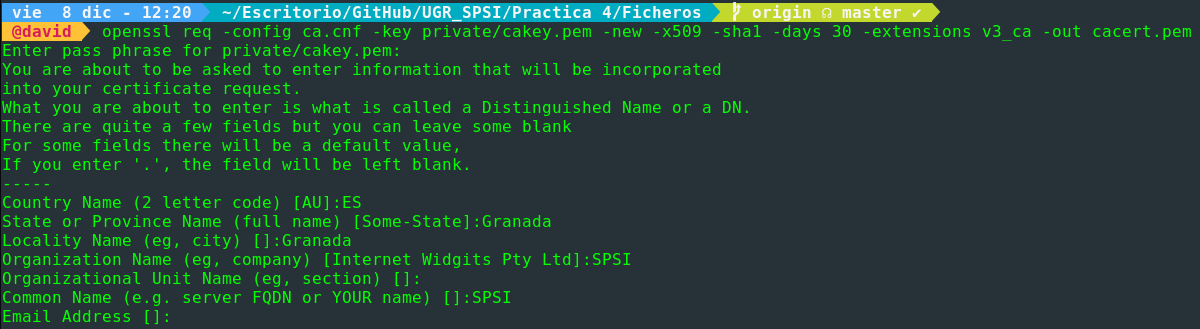
\includegraphics[width=1\textwidth]{./Imagenes/1_4.png}
\end{figure}

\noindent
Con esto ya tenemos listo el certificado que usará nuestra autoridad certificadora.

% ----------------------------------------------------------------
\chapter{Ejercicio 2}

\section{Enunciado}
\noindent
Cread una solución de certificado que incluya la generación de claves en la misma.

\section{Respuesta}
\noindent

\begin{figure}[!hbp]
 \centering  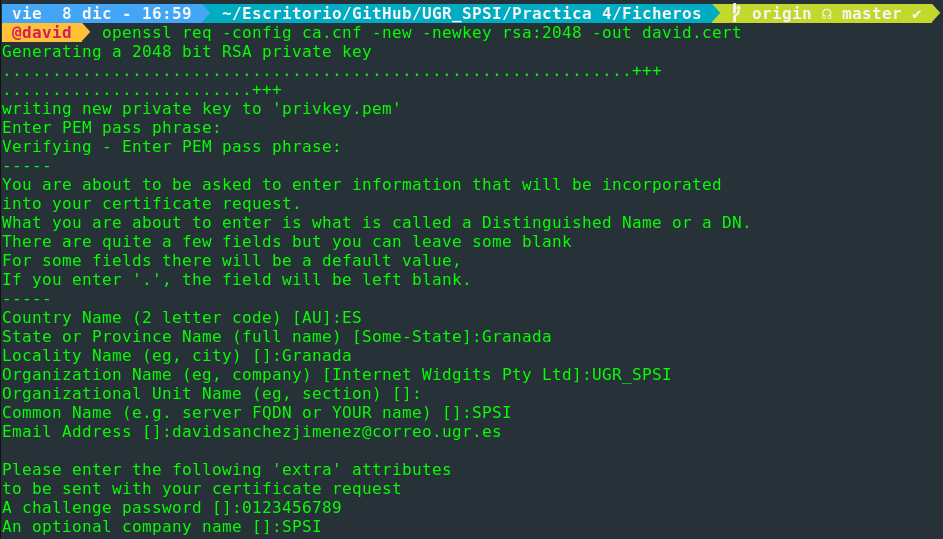
\includegraphics[width=1\textwidth]{./Imagenes/2.png}
\end{figure}

% ----------------------------------------------------------------
\chapter{Ejercicio 3}

\section{Enunciado}
\noindent
Cread un certificado para la solicitud anterior empleando la CA creada en el primer punto.

\section{Respuesta}
\noindent

% ----------------------------------------------------------------
\chapter{Ejercicio 4}

\section{Enunciado}
\noindent
Cread una solicitud de certificado para cualquiera de las claves que habéis generado en las prácticas anteriores, excepto las RSA.

\section{Respuesta}
\noindent

% ----------------------------------------------------------------
\chapter{Ejercicio 5}

\section{Enunciado}
\noindent
Cread un certificado para la solicitud anterior utilizando la CA creada.

\section{Respuesta}
\noindent

% ----------------------------------------------------------------
\chapter{Ejercicio 6}

\section{Enunciado}
\noindent
Emplead las opciones -text y -noout para mostrar los valores de todos los certificados y solicitudes de los puntos anteriores, incluyendo el certificado raíz que habrá sido creado junto con la CA.

\section{Respuesta}
\noindent

% ----------------------------------------------------------------

\end{document}
